% COMPOSITE

\subsection{Problem Set}

\subsubsection{(Problem 1) PSS 1.1 Motion Diagrams}
~
\begin{prb}

	A car is traveling with constant velocity along a highway. The driver notices he is late for work, so he stomps down on the gas pedal and the car begins to speed up. The car has just achieved double its initial velocity when the driver spots a police officer behind him and applies the brakes. The car then slows down, coming to rest at a stoplight ahead.

	Draw a complete motion diagram for this situation.

\end{prb}

\footnote{Cont. on next page}

\newpage

\subsubsection{Part A}

The car's motion can be divided into three different stages: its motion before the driver realizes he's late, its  motion after the driver hits the gas (but before he sees the police car), and its motion after the driver sees the police car. Which of the following simplifying assumptions is it reasonable to make in this problem?

\vspace{1em}

\begin{solution}
	I selected the following options:

	\begin{enumerate}
		\item During each of the three different stages of its motion, the car is moving with constant acceleration.
		\item The highway is straight (i.e., there are no curves).
		\item The highway is level (i.e., there are no hills or valleys).
	\end{enumerate}

	These are reasonable assumptions to make for the diagram, as no further constraints were given in the original problem.

\end{solution}

\begin{center}
	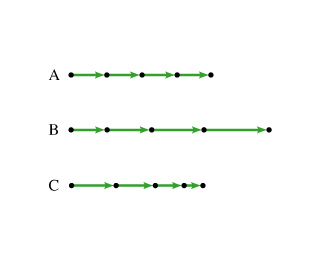
\includegraphics[width=0.5\textwidth]{"/Users/max/course-manager/data/semester/Spring 2025/course/PHY2111/chapter/Concepts of Motion/section/1.1-1.8/figures/diagram_1.jpg"}
\end{center}

\subsubsection{Part B}
In the three diagrams shown [above], the position of the car at five subsequent instants of time is represented by black dots, and the car's average velocity is represented by green arrows. Which of these diagrams best describes the position and the velocity of the car before the driver notices he is late?

\vspace{1em}

\begin{solution}
	I selected diagram $A$, as it depicts the car moving with constant velocity and no acceleration, as described by the problem.
\end{solution}

\subsubsection{Part C}
Which of the diagrams shown [above] best describes the position and the velocity of the car after the driver hits the gas, but before he notices the police officer?

\vspace{1em}

\begin{solution}
	I selected diagram $B$, as it depicts the car accelerating. The dots increase in distance at each time interval.
\end{solution}

\subsubsection{Part D}
Which of the diagrams shown to the left best describes the position and the velocity of the car after the driver notices the police officer?

\vspace{1em}

\begin{solution}
	I selected diagram $C$, as it depicts the car decelerating, which aligns with the scenario outlined in the problem.
\end{solution}

\subsubsection{Part E}
Which of the diagrams shown below most accurately depicts the average acceleration vectors of the car during the events described in the problem introduction?

\begin{center}
	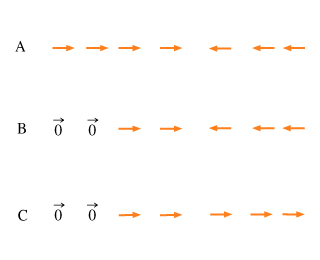
\includegraphics[width=0.5\textwidth]{"/Users/max/course-manager/data/semester/Spring 2025/course/PHY2111/chapter/Concepts of Motion/section/1.1-1.8/figures/diagram_2.jpg"}
\end{center}

\vspace{1em}

\begin{solution}
	I chose diagram $B$, as it depicts the car's acceleration appropriately:
	\begin{enumerate}
		\item The car starts with zero acceleration,
		\item the driver accelerates (indicated by the right-facing arrows),
		\item and decelerates (indicated by the left-facing arrows).
	\end{enumerate}
\end{solution}

\begin{center}
	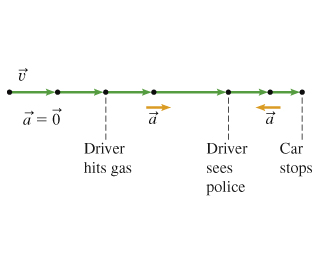
\includegraphics[width=0.5\textwidth]{"/Users/max/course-manager/data/semester/Spring 2025/course/PHY2111/chapter/Concepts of Motion/section/1.1-1.8/figures/diagram_3.jpg"}
\end{center}

\newpage

\subsubsection{(Problem 2) Conceptual Question 1.6}

\begin{center}
	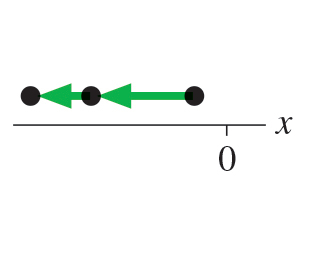
\includegraphics[width=0.5\textwidth]{"/Users/max/course-manager/data/semester/Spring 2025/course/PHY2111/chapter/Concepts of Motion/section/1.1-1.8/figures/diagram_4.jpg"}
\end{center}

\subsubsection{Part A, B, C}
Determine the sign (positive, negative, or zero) of the position, velocity, and acceleration for the particle [in the diagram above]

\vspace{1em}

\begin{solution}
	\begin{enumerate}
		\item The sign of the particle's position is \textbf{negative}, since the three depicted positions are to the left of the origin.
		\item The sign of the particle's velocity is \textbf{negative}, since the arrows point to the left of the origin.
		\item The sign of the particle's acceleration is \textbf{positive}, since the distance between the points decreases over time. This can only be explained by an acceleration vector in the opposite direction of the velocity.
	\end{enumerate}
\end{solution}

\newpage

\subsubsection{(Problem 3) Conceptual Question 1.7}

\begin{center}
	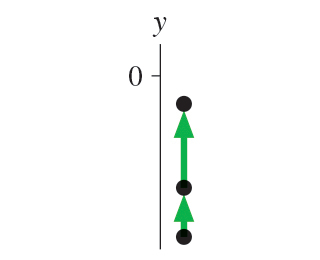
\includegraphics[width=0.5\textwidth]{"/Users/max/course-manager/data/semester/Spring 2025/course/PHY2111/chapter/Concepts of Motion/section/1.1-1.8/figures/diagram_5.jpg"}
\end{center}

\subsubsection{Part A, B, C}
Determine the sign (positive, negative, or zero) of the position, velocity, and acceleration for the particle [in the diagram above]

\vspace{1em}

\begin{solution}
	\begin{enumerate}
		\item The sign of the particle's position is \textbf{negative}, since the three depicted positions are below the origin.
		\item The sign of the particle's velocity is \textbf{positive}, since the arrows point upwards.
		\item The sign of the particle's acceleration is \textbf{positive}, since the distance between the points increases over time. This can only be explained by an acceleration vector in the same direction of the velocity.
	\end{enumerate}
\end{solution}

\newpage

\subsubsection{(Problem 4) Problem 1.2 - Enhanced - with Hints and Feedback}

You are watching a jet ski race. A racer speeds up from rest to 70 mph in just a few seconds, then continues at a constant speed.

\subsubsection{Part A}
Select the correct basic motion diagram of the jet ski, using images from the video, from $10s$ before reaching top speed until $10s$ afterward.

\vspace{1em}

\begin{solution}

	I chose the following diagram:

	\begin{center}
		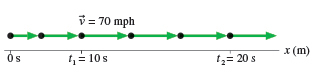
\includegraphics[width=0.5\textwidth]{"/Users/max/course-manager/data/semester/Spring 2025/course/PHY2111/chapter/Concepts of Motion/section/1.1-1.8/figures/diagram_6.jpg"}
	\end{center}

	since it accurately depicts the motion of the jet ski as described.

\end{solution}

\newpage

\subsubsection{(Problem 5) Problem 1.16 - Enhanced - with Expanded Hints}

A roof tile falls straight down from a two-story building. It lands in a swimming pool and settles gently to the bottom.

Select the correct complete motion diagram of the tile.

\vspace{1em}

\begin{solution}

	I chose the following diagram:

	\begin{center}
		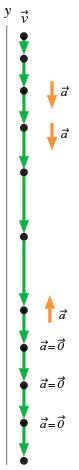
\includegraphics[height=0.5\textwidth]{"/Users/max/course-manager/data/semester/Spring 2025/course/PHY2111/chapter/Concepts of Motion/section/1.1-1.8/figures/diagram_7.jpg"}
	\end{center}

	since it accurately depicts the motion of the roof tile as described.
\end{solution}

\newpage

\subsubsection{(Problem 6) $\pm$ Scientific Notation}

A number written in scientific notation has the form $a \times 10^{k}$, where $1 \le a < 10$ and $k$ is an integer, that is, $k$ is one of $\ldots -3, -2, -1, 0, 1, 2, 3 \ldots$

\subsubsection{Part A}
Determine the values of $a$ and $k$ when $299{\small,}790{\small,}000$ is written in scientific notation.

\vspace{1em}

\begin{solution}
	Since scientific notation requires $a$ to be less than $10$, we can shift the decimal place $8$ digits to the left, meaning that
	\begin{align*}
		a &= 2.9979 \\
		k &= 8 \\
		a \times 10^{k} &= 2.9979 \times 10^{8}
		.\end{align*}
\end{solution}

\subsubsection{Part B}
Determine the values of $a$ and $k$ when $0.51$ is written in scientific notation.

\vspace{1em}

\begin{solution}
	\begin{align*}
		a &= 5.1 \\
		k &= -1 \\
		a \times 10^{k} &= 5.1 \times 10^{-1}
		.\end{align*}
\end{solution}

\subsubsection{Part C}
Now consider the expression $4.0 \times 10^{3} + 4 \times 10^2$. Determine the values of $a$ and $k$ when this expression is written in scientific notation.

\vspace{1em}

\begin{solution}
	\begin{align*}
		\left( 4.0 \times 10^{3} \right) + \left( 4 \times 10^2 \right) &=
		\left( 4000 \right) + \left( 400 \right) \\
		&= 4400
	\end{align*}
	\begin{align*}
		a &= 4.4 \\
		k &= 3 \\
		a \times 10^{k} &= 4.4 \times 10^{3}
	\end{align*}
\end{solution}

\subsubsection{Part D}

Finally, consider the expression
\[
	\frac{\left( 6.67 \times 10^{-11} \right)\left( 5.97 \times 10^{24} \right)}{\left( 6.38 \times 10^{6} \right)^2}
	.\]
Determine the values of $a$ and $k$ when the value of this expression is written in scientific notation.

\vspace{1em}

\begin{solution}
	\begin{align*}
		\frac{\left( 6.67 \times 10^{-11} \right)\left( 5.97 \times 10^{24} \right)}{\left( 6.38 \times 10^{6} \right)^2} &=
		\frac{\left( 6.67 \times 5.97 \right) \times 10^{13}}{\left( 40.7044 \times 10^{12} \right)} \\
		&= \frac{39.8199 \times 10^{13}}{40.7044 \times 10^{12}} \\
		&= 0.978270 \times 10^{1} \\
		&= 9.78270 \times 10^{0} \\
	\end{align*}
	\begin{align*}
		a &= 9.78270 \\
		k &= 0
		.\end{align*}
\end{solution}

\newpage

\subsubsection{(Problem 7) Converting Units: The Magic of 1}

\subsubsection{Part A}
How many centimeters are there in a length $25.9$ inches? Express your answer in centimeters to three significant figures.

\vspace{1em}

\begin{solution}
	Since there are $2.54$ centimeters per inch,
	\begin{align*}
		x~\text{cm} &= 25.9 \cdot 2.54 \\
		&= 65.786~\text{cm} \\
		&= 65.8~\text{cm}
		.\end{align*}
\end{solution}

\subsubsection{Part B}
Suppose that a particular artillery piece has a range $R=9070$ yards. Find its range in miles. Use the facts that $1$ mile $= 5280$ ft and $3$ feet $= 1$ yard. Express your answer in miles to three significant figures.

\vspace{1em}

\begin{solution}
	\begin{align*}
		9070~\text{yards} &= \left( 3 \cdot 9070 \right)~\text{feet} = 27210~\text{feet} \\
		\frac{27210~\text{feet}}{5280~\text{feet}} &= 5.15340909~\text{miles} \\
		R &= 5.15~\text{miles}
		.\end{align*}
\end{solution}

\subsubsection{Part C}
What is the speed of a car going $v=1.000$mph in SI units? Notice that you will need to change from miles to meters and from hours to seconds. You can do each conversion separately. Use the facts that $1$ mile $= 1609$ meters and $1$ hour $= 3600$ seconds.

\begin{solution}
	\begin{align*}
		1~\text{mile} &= 1609~ \text{meters} \\
		\frac{1609~\text{meters}}{3600~\text{seconds}} &\approx 0.4469~\text{m/s}
		.\end{align*}
\end{solution}

\newpage

\subsubsection{(Problem 8) Problem 1.24 - Enhanced - with Expanded Hints}

Convert the following to basic SI units or a combination of basic SI units:

\subsubsection{Part A}

$11$ inches. Express your answer with the appropriate units.

\begin{solution}
	\begin{align*}
		11~\text{inches} &= 11 \cdot 2.54 = 27.94~\text{cm} \\
		\frac{27.94~\text{cm}}{100~\text{cm}} &= 0.2794~\text{meters}
		.\end{align*}
\end{solution}

\subsubsection{Part B}

$66$ ft/s. Express your answer with the appropriate units.

\vspace{1em}

\begin{solution}
	\begin{align*}
		66~\text{feet} &= 66 \cdot 12 = 792~\text{inches} \\
		\frac{792~\text{inches}}{39.37~\text{inches}} &\approx 20~\text{m/s}
		.\end{align*}
\end{solution}

\subsubsection{Part C}

$85$ mph. Express your answer with the appropriate units.

\vspace{1em}

\begin{solution}
	\begin{align*}
		85~\text{miles} &= 85 \cdot 1.609 = 136.765~\text{kilometers} \\
		136.765~\text{kilometers} &= 136.765 \cdot 1000 = 136765~\text{meters} \\
		\frac{136765~\text{meters}}{3600~\text{seconds}} &\approx 38~\text{m/s}
		.\end{align*}
\end{solution}

\subsubsection{Part D}

$22~\text{in}^2$. Express your answer with the appropriate units.

\vspace{1em}

\begin{solution}
	\begin{align*}
		\left( 22~\text{in}^2 \right) \left( \frac{1~\text{m}}{39.37~\text{in}} \right)^2
		&= 22~\text{in}^2 \cdot \frac{1}{1549.9969~\text{in}^2} \\
		&= \frac{22~\text{in}^2}{1549.9969~\text{in}^2} \\
		&= 0.01419358~\text{in}^2 \\
		&\approx 1.4 \times 10^{-2}~\text{m}^2
		.\end{align*}
\end{solution}

\newpage

\subsubsection{(Problem 9) Problem 1.27 - Enhanced - with Expanded Hints}

Using the approximate conversion factors listed below, convert the following SI units to English without using your calculator.

\begin{center}
	\begin{tblr}{c|c}
		metric & imperial \\
		\hline
		10 cm  & 4 in     \\
		1 m    & 1 yard   \\
		1 m    & 3 feet   \\
		1 km   & 0.6 mile \\
		1 m/s  & 2 mph
	\end{tblr}
\end{center}

\subsubsection{Part A}

50 cm. Express your answer in inches.

\vspace{1em}

\begin{solution}
	\begin{align*}
		4~\text{in} \cdot 5 &= 20~\text{in}
		.\end{align*}
\end{solution}

\subsubsection{Part B}

22 m/s. Express your answer in miles per hour.

\vspace{1em}

\begin{solution}
	\begin{align*}
		22~\text{m/s} \cdot 2 &= 44~\text{mph}
		.\end{align*}
\end{solution}

\subsubsection{Part C}

5 km. Express your answer in miles.

\vspace{1em}

\begin{solution}
	\begin{align*}
		5~\text{km} \cdot \left( \frac{0.6~\text{mile}}{1~\text{km}} \right) &= 3~\text{miles}
		.\end{align*}
\end{solution}

\subsubsection{Part D}

0.5 cm. Express your answer in inches.

\vspace{1em}

\begin{solution}
	\begin{align*}
		0.5~\text{cm} \left( \frac{0.4~\text{in}}{1~\text{cm}} \right) &= 0.2~\text{inches}
		.\end{align*}
\end{solution}

\subsubsection{(Problem 10) Conceptual Question 1.2}

How many significant figures does each of the following numbers have?

\subsubsection{Part A, B, C, D}

\vspace{1em}

\begin{solution}
	\begin{enumerate}[label=\Alph*.]
		\item $8.70 \to 3$ significant figures
		\item $8.7 \times 10^{5} \to 2$ significant figures
		\item $870 \to 2$ significant figures
		\item $0.0087 \to 2$ significant figures
	\end{enumerate}
\end{solution}

\subsubsection{(Problem 11) Problem 1.29 - Enhanced - with Expanded Hints}

Compute the following numbers, applying the significant figure rule adopted in this textbook.

\subsubsection{Part A, B, C, D}

\begin{solution}
	\begin{enumerate}[label=\Alph*.]
		\item $34.1 \times 24.9 = 849.09 \approx 849$
		\item $34.1 - 24.9 = 9.2$
		\item $\sqrt{34.1} = 5.83952053 \approx 5.84$
		\item $\frac{333.3}{24.9} = 13.38554217 \approx 13.4$
	\end{enumerate}
\end{solution}

\newpage

\subsubsection{(Problem 12) Problem 1.53 - Enhanced - with Hints and Feedback}

As an architect, you are designing a new house. A window has a height between 150 cm and 160 cm and a width between 72 cm and 60 cm.

\subsubsection{Part A}

What is the smallest area that the window could be? Express your answer with the appropriate units and with the appropriate number of significant figures.

\vspace{1em}

\begin{solution}
	\begin{align*}
		A_{\text{min}} &= w_{\text{min}} \cdot h_{\text{min}} \\
		A_{\text{min}} &= 60~\text{cm} \cdot 150~\text{cm} \\
		&= 9000~\text{cm}^2
		.\end{align*}
\end{solution}

\subsubsection{Part B}

What is the smallest area that the window could be? Express your answer with the appropriate units and with the appropriate number of significant figures.

\vspace{1em}

\begin{solution}
	\begin{align*}
		A_{\text{max}} &= w_{\text{max}} \cdot h_{\text{max}} \\
		A_{\text{max}} &= 72~\text{cm} \cdot 160~\text{cm} \\
		&= 11520~\text{cm}^2 \\
		&\approx 1.15 \times 10^{4}~\text{cm}^2
		.\end{align*}
\end{solution}

\newpage

\subsubsection{(Problem 13) Problem 1.55 - Enhanced - with Video Tutor Solution}

A 4.5-cm-diameter cylinder has a length of 11.5 cm.

\subsubsection{Part A}

What is the cylinder's volume in basic SI units? Express your answer with the appropriate units and with the appropriate number of significant figures.

\vspace{1em}

\begin{solution}
	\begin{align*}
		V_{\text{cylinder}} &= \pi r^2 h \\
		V_{\text{cylinder}} &= \pi \left( \frac{0.045~\text{meter}}{2} \right)^2 \left( 0.115~\text{meter} \right) \\
		&= \pi \left( 0.0225~\text{meter} \right)^2 \left( 0.115~\text{meter} \right) \\
		&= \pi \left( 0.00050625~\text{meter}^2 \right) \left( 0.115~\text{meter} \right) \\
		&= 0.0001829~\text{m}^3 \\
		&\approx 1.8 \times 10^{-4}~\text{m}^3
		.\end{align*}
\end{solution}

\newpage

\subsubsection{Part A}

Does the object represented in the figure below have positive or negative value of $a_{x}$? Explain. Assume that the $x$-axis points to the right. Match the words in the left column to the appropriate blanks in the sentences on the right.

\begin{center}
	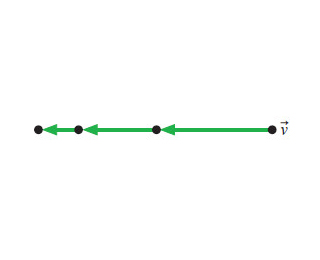
\includegraphics[width=0.5\textwidth]{"/Users/max/course-manager/data/semester/Spring 2025/course/PHY2111/chapter/Concepts of Motion/section/1.1-1.8/figures/diagram_8.jpg"}
\end{center}

\begin{solution}
	The object has a positive acceleration $a_x$ (in the opposite direction of $v_x$), since it is slowing down over time.
\end{solution}

\newpage

\subsubsection{(Problem 15) General Problem-Solving Strategy}

Two hockey pucks, labeled $A$ and $B$, are initially at rest on a smooth ice surface and are separated by a distance of 18.0 m. Simultaneously, each puck is given a quick push, and they begin to slide directly toward each other. Puck $A$ moves with a speed of 4.10 m/s, and puck $B$ moves with a speed of 7.50 m/s.

What is the distance covered by puck $A$ by the time the two pucks collide?

\subsubsection{Part A}

Which of the motion diagrams shown here best represents the motion of puck A prior to the collision?

\begin{center}
	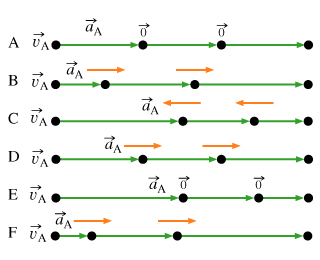
\includegraphics[width=0.5\textwidth]{"/Users/max/course-manager/data/semester/Spring 2025/course/PHY2111/chapter/Concepts of Motion/section/1.1-1.8/figures/diagram_9.jpg"}
\end{center}

\begin{solution}
	I chose diagram $A$, since it depicts the scenario the most accurately. In the real world there would be friction (resulting in an acceleration vector pointing in the direction opposite of the motion of the puck), but this is an appropriate simplification.
\end{solution}

\subsubsection{Part B}

After completing your motion diagram, it's time to choose an appropriate coordinate system for this problem. Note that there is no single correct way to visualize this problem, but for the questions that follow, assume that the pucks are moving along the $x$ axis with $+x$ directed to the right. Take the initial position of puck $A$, when it is at rest, to be at the origin, and take the initial position of puck $B$ to be to the right of puck $A$. Start your clock at the instant when the pucks begin to move.

Based on the assumptions listed above, sort the following quantities as known or unknown.
Drag the appropriate items to their respective bins.

\vspace{1em}

\begin{solution}~

	\begin{center}
		\begin{tabular}{p{13em}|p{13em}}
			Known                                           & Unknown                                             \\
			\hline
			the initial position of puck $A$                & the moment of collision                             \\
			the initial position of puck $B$                & the position of puck $A$ at the moment of collision \\
			the initial time (when the pucks begin to move) & the position of puck $B$ at the moment of collision \\
			the initial velocity of puck B                  &
		\end{tabular}
	\end{center}

\end{solution}

\subsubsection{Part C}

Which of the following relationships follows from the problem statement?

Note that $\left( x_1 \right)_{A}$  and $\left( x_1 \right)_{B}$ are the positions of the pucks at the moment of their collision.

\vspace{1em}

\begin{solution}
	I chose the following relationship:
	\[
		\left( x_1 \right)_{A} = \left( x_1 \right)_{B}
	\]
	because, at the moment of collision, the pucks would need to be at the same position (in the simplified model where the pucks have no width).
\end{solution}

\subsubsection{Part D}

What is $x_1$, the distance that puck $A$ covers prior to the collision?
Express your answer in meters to three significant figures. Do not include units in your answer.

\vspace{1em}

\begin{solution}
	Given
	\begin{align*}
		\left( x_1 \right)_{A} &= 0~\text{m}+4.10~\text{m/s} \cdot t_1 \\
		\left( x_1 \right)_{B} &= 18.0~\text{m} - 7.50~\text{m/s} \cdot t_1 \\
		\left( x_1 \right)_{A} &= \left( x_1 \right)_{B}
		,\end{align*}

	We can solve for $t_1$ by setting the equations equal to each other.
	\begin{align*}
		4.10~\text{m/s} \cdot t_1 &= 18.0~\text{m} - 7.50~\text{m/s} \cdot t_1 \\
		18.0~\text{m} &= 4.10~\text{m/s} * t_1 + 7.50~\text{m/s} * t_1 \\
		18.0~\text{m} &= t_1 \left( 4.10~\text{m/s} + 7.50~\text{m/s} \right) \\
		\frac{18.0~\text{m}}{11.6~\text{m/s}} &= t_1 \\
		t_1 &= 1.55172414~\text{s} \\
		.\end{align*}

	Finally, we can determine $x_1$ by multiplying $t_1$ by the velocity of puck $A$:
	\begin{align*}
		x_1 &= t_1 \cdot \left( v_{0_{x}} \right)_{A} \\
		x_1 &= 1.55172414~\text{s} \cdot 4.10~\text{m/s} \\
		&\approx 6.36~\text{m}
		.\end{align*}
\end{solution}

\subsubsection{Part E}

Your answer should satisfy common sense. For instance, can you decide which of the following values for the distance covered by puck A would definitely be wrong, regardless of the speed of the two pucks and considering that the two pucks are sliding toward each other?

\vspace{1em}

\begin{solution}
	I chose the following options:
	\begin{enumerate}
		\item 19 m
		\item 25 m
	\end{enumerate}
	because these values are greater than the initial distance of the two pucks, implying that the collision happens at an impossible distance.
\end{solution}

\newpage

\subsubsection{(Problem 16) Problem 1.52 - Enhanced - with Hints and Feedback}

\begin{center}
	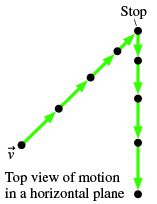
\includegraphics[height=0.3\textwidth]{"/Users/max/course-manager/data/semester/Spring 2025/course/PHY2111/chapter/Concepts of Motion/section/1.1-1.8/figures/diagram_10.jpg"}
\end{center}

\subsubsection{Part A}

Select the correct motion diagram with added acceleration vector. A partial motion diagram is shown in the figure above.

\vspace{1em}

\begin{solution}
	I chose the following diagram:
	\begin{center}
		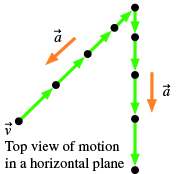
\includegraphics[height=0.3\textwidth]{"/Users/max/course-manager/data/semester/Spring 2025/course/PHY2111/chapter/Concepts of Motion/section/1.1-1.8/figures/diagram_11.jpg"}
	\end{center}
	because it depicts the acceleration vectors accurately, as the particle is slowing down and then speeding up.
\end{solution}

\subsubsection{Part B}

Select the correct physics problem for which this is the correct motion diagram.

\vspace{1em}

\begin{solution}
	I chose the following option:

	"Jeremy has perfected the art of steady acceleration and deceleration. From a speed of 60 mph  he brings his car to a halt in 10 s with a constant magnitude of deceleration. Then he turns into an adjoining street. Starting from rest, Jeremy accelerates with exactly the same magnitude as his earlier magnitude of deceleration and reaches the same speed of 60 mph over the same distance in exactly the same time. Find the car's acceleration or deceleration."

	This option suits the diagram because it aligns with the acceleration and deceleration; they appear to be consistent but opposite of each other, and him turning onto "an adjoining street" matches the velocity direction change.
\end{solution}

\subsubsection{Part C}

Select the correct pictorial representation for your problem.

\vspace{1em}

\begin{solution}
	I chose the following representation:
	\begin{center}
		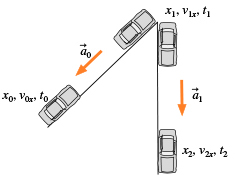
\includegraphics[height=0.4\textwidth]{"/Users/max/course-manager/data/semester/Spring 2025/course/PHY2111/chapter/Concepts of Motion/section/1.1-1.8/figures/diagram_12.jpg"}
	\end{center}
	\begin{center}
		\[
			\begin{tblr}{c}
				\text{Known} \\
				\hline
				v_{0_{x}} = 60~\text{mph} \\
				t_0 = 0~\text{s} \\
				x_0 = 0~\text{m} \\
				v_{1_{x}} = 0 \\
				t_1 = 10~\text{s} \\
				v_{2_{x}} = 60~\text{mph} \\
				t_2 = 20~\text{s} \\
				x_2 = 2x_1
			\end{tblr}
		\]
		This aligns with the problem because the known variables correspond with the equivalent starting and ending speeds.
	\end{center}
\end{solution}
